% arXiv-ready LaTeX — two-column, 10pt, CS conference style
\documentclass[10pt,twocolumn]{article}

% ---------- packages ----------
\usepackage[utf8]{inputenc}
\usepackage[T1]{fontenc}
\usepackage{times}                     % standard CS conference font
\usepackage[margin=0.75in]{geometry}   % tight but readable margins
\usepackage{graphicx}
\usepackage{booktabs}
\usepackage{amsmath,amssymb}
\usepackage{url}
\usepackage[colorlinks,citecolor=blue,urlcolor=blue,linkcolor=black]{hyperref}
\usepackage{tikz}
\usetikzlibrary{positioning,arrows.meta,calc,patterns,decorations.pathreplacing}
\usepackage{caption}
\usepackage{subcaption}
\usepackage{enumitem}
\usepackage{xcolor}
\usepackage{microtype}
\usepackage{natbib}
\bibliographystyle{plainnat}

% ---------- compact spacing ----------
\setlength{\columnsep}{0.25in}
\setlength{\parskip}{0pt}
\setlength{\abovecaptionskip}{6pt}
\setlength{\belowcaptionskip}{2pt}
\renewcommand{\baselinestretch}{0.97}

% convenience
\newcommand{\ie}{\emph{i.e.}}
\newcommand{\eg}{\emph{e.g.}}
\newcommand{\x}{\times}

% ---------- title ----------
\title{Heterogeneous Tensor Parallelism over Commodity TCP Networks\\via FP32 GPU-Native Reduction}

\author{Brian Habana\\
  BareMetalRT\\
  \texttt{brian@baremetalrt.com}}

\date{}

\begin{document}
\maketitle

% ============================================================
\begin{abstract}
We present the first system that achieves \textbf{heterogeneous tensor
parallelism on ad-hoc consumer GPUs over commodity TCP networks}, running
Mistral 7B---a 14\,GB model too large for either GPU alone---across an
RTX~4070 Super (12\,GB) and an RTX~4060 Laptop (8\,GB) at
\textbf{80\,ms/token (12.5\,tok/s)}.  Every prior distributed inference
project on consumer hardware chose pipeline parallelism, accepting idle
GPUs and architectural limitations as unavoidable.  Data-center systems
(HexGen, Helix) support heterogeneous tensor parallelism but require
managed clusters, Linux, and offline profiling.

The central contribution is a precision result: FP32 end-to-end computation
achieves the \textbf{theoretical floor} of IEEE~754 single-precision
arithmetic---identical to NCCL on NVLink and $2{,}500\times$ more accurate
than FP16.  No implementation of tensor parallelism at FP32 precision, on
any hardware, can do better.  An
asymmetric-tolerant TCP transport replaces NCCL, enabling GPUs with
different VRAM and compute capabilities to participate in the same
AllReduce without barrier stalls or protocol-level assumptions of symmetric
hardware.  The system is built on NVIDIA TensorRT-LLM ported natively to
Windows.

Our benchmarks reveal a counterintuitive finding: in synchronous tensor
parallelism, \textbf{GPU synchronization overhead---not network
latency---is the dominant bottleneck}.  A $300\times$ improvement in
network speed (WiFi to ethernet) yielded zero throughput improvement.  We
argue that Mixture-of-Experts architectures structurally favor distributed
meshes over centralized data centers, replacing dense AllReduce with sparse
expert routing over commodity networks.
\end{abstract}

% ============================================================
\section{Introduction}\label{sec:intro}

A 7-billion-parameter model doesn't fit on most consumer GPUs.
A 70-billion-parameter model doesn't fit on \emph{any} of them.
But most households with a gaming PC have more than enough aggregate VRAM
across machines to run these models---if those GPUs could work together.
They can't.  Over 100 million RTX-class NVIDIA GPUs sit in PCs and
workstations~\citep{nvidia2024rtx}, and almost none of them can combine
their memory and compute with the GPU in the next room, let alone across a
network.

This isn't a missing feature---it's a missing \emph{category}.
Every existing path forces a choice between quality and accessibility.
Cloud inference (OpenAI, Anthropic, Google) uses data-center-grade hardware
with optimized kernels---but is expensive, rate-limited, and geographically
constrained.  Local inference tools (Ollama, LM~Studio, Jan, GPT4All) run
on consumer hardware---but are limited to a single machine, use a
general-purpose CUDA backend that leaves significant performance on the
table, and can only run models that fit in one GPU's memory.  Distributed
inference projects (Petals~\citep{borzunov2023petals},
Exo~\citep{exo2024}) can span multiple machines---but only via pipeline
parallelism, which wastes half the available compute to pipeline bubbles
and limits model architectures.  The fastest inference
kernels---NVIDIA's TensorRT-LLM~\citep{nvidia2024trtllm}, with 1,500+
hand-optimized CUDA routines---exist, but require homogeneous data-center
GPUs communicating over NVLink or InfiniBand via
NCCL~\citep{nvidia2024nccl}.

No system combines the three things needed at once: \textbf{optimized
kernels} that extract full performance from the hardware, \textbf{tensor
parallelism} that keeps every GPU busy on every layer, and
\textbf{heterogeneous support} that lets different GPUs with different VRAM
and different compute capabilities---on different machines, over a
commodity network---contribute to a single inference pass.
That is the problem this paper solves.
Moreover, the industry's shift toward Mixture-of-Experts (MoE)
architectures---which activate only a fraction of parameters per
token---creates a structural advantage for distributed meshes over
centralized data centers, a direction we explore in
\S\ref{sec:future}.

% ============================================================
\section{Related Work}\label{sec:related}

\paragraph{Parallelism strategies.}
Model parallelism for large neural networks has been explored along two
axes.  Pipeline parallelism (PP), introduced by
GPipe~\citep{huang2019gpipe}, partitions a model into sequential stages
assigned to different devices.  Megatron-LM~\citep{shoeybi2019megatron}
introduced intra-layer tensor parallelism (TP) for transformer models,
splitting attention and MLP layers horizontally across GPUs connected by
NVLink within a single DGX node.  DeepSpeed~\citep{rasley2020deepspeed}
combines PP with ZeRO-style memory optimization for training at scale.
Alpa~\citep{zheng2022alpa} automates the selection of inter- and
intra-operator parallelism strategies via ILP\@.  All of these systems
assume homogeneous hardware within each parallelism group and rely on
NCCL~\citep{nvidia2024nccl} for collective communication---requiring
Linux, NVLink or InfiniBand, and identical GPUs.

\paragraph{Distributed inference on consumer hardware.}
Petals~\citep{borzunov2023petals} enables collaborative inference by
distributing transformer blocks across volunteers over the internet, using
pipeline parallelism exclusively.  The authors explicitly state that tensor
parallelism is infeasible in their setting due to per-layer activation
transfers.  Exo~\citep{exo2024} similarly builds on pipeline parallelism
for home clusters, acknowledging that inter-device latency makes per-layer
synchronization impractical.  Both systems accept pipeline bubbles and
sequential stage execution as necessary tradeoffs.  Neither supports
heterogeneous GPUs within a parallelism group, and neither addresses the
precision loss that occurs when AllReduce is performed over a network
rather than NVLink.

\paragraph{Offloading and single-GPU approaches.}
FlexGen~\citep{sheng2023flexgen} enables large model inference on a single
GPU by offloading weights to CPU and disk, trading latency for
accessibility.  \texttt{llama.cpp} provides CPU and CUDA inference via a
general-purpose backend but does not use TensorRT-LLM's optimized kernels
and does not support multi-machine parallelism.  These approaches are
complementary: they maximize single-device utilization, while our work
enables models too large for any single device.

\paragraph{Heterogeneous parallelism.}
AMP~\citep{lee2022amp} explores asymmetric partitioning for training on
heterogeneous GPU clusters, assigning different numbers of layers to
devices based on compute capability---a form of asymmetric pipeline
parallelism, not tensor parallelism.  HexGen~\citep{jiang2024hexgen}
supports asymmetric tensor and pipeline parallelism over heterogeneous GPUs
and networks, using constrained optimization to assign workloads
proportionally to device capability.  Helix~\citep{mei2025helix}
formulates heterogeneous LLM serving as a max-flow problem over weighted
GPU graphs.  Both achieve significant throughput improvements over
homogeneous baselines---but both assume managed datacenter clusters with
known topology, require offline profiling and optimization passes, and
build on existing Linux-only frameworks (vLLM, Megatron).  Neither targets
ad-hoc consumer hardware, WiFi or commodity TCP networks, or Windows.  Our
work demonstrates heterogeneous tensor parallelism in the setting these
systems explicitly do not address: consumer GPUs with different VRAM and SM
counts, discovered dynamically, communicating over commodity TCP without
NVLink or InfiniBand---and does so with FP32-accurate AllReduce that
prevents the precision loss inherent in networked reduction.

% ============================================================
\section{Approach: FP32 Reduction and Asymmetric Tensor Parallelism}\label{sec:approach}

Every prior attempt at distributed LLM inference over consumer hardware
chose pipeline parallelism---and accepted the bubbles, idle GPUs, and
architectural limitations that come with it.  Tensor parallelism was
considered infeasible outside of homogeneous data center hardware.  Our
system solves the two problems that blocked it: \textbf{precision loss
during networked AllReduce}, and \textbf{synchronization failure across
mismatched GPUs}.  Together, they enable heterogeneous tensor parallelism
on consumer hardware over commodity networks---a setting no prior system
has addressed.

As described in \S\ref{sec:related}, pipeline parallelism
(PP)~\citep{huang2019gpipe} splits models vertically across stages, while
tensor parallelism (TP)~\citep{shoeybi2019megatron} splits each layer
horizontally, keeping every GPU active on every layer.  TP requires
AllReduce synchronization at every layer boundary---and every existing
implementation assumes identical GPUs.

% ---------- Figure 1: PP vs TP ----------
\begin{figure}[t]
\centering
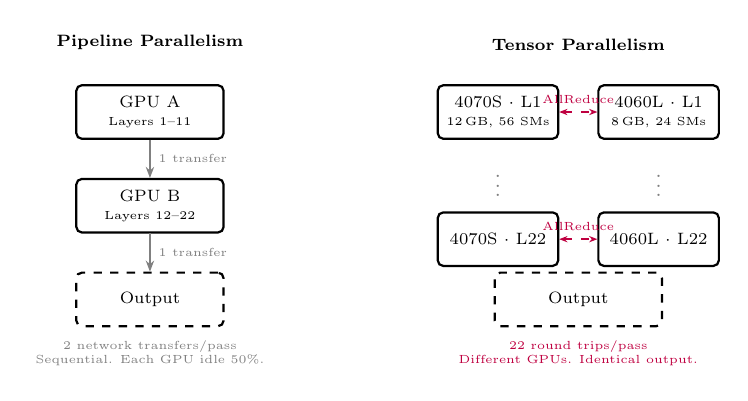
\begin{tikzpicture}[
    box/.style={draw, rounded corners=2pt, minimum width=2.2cm, minimum height=0.8cm,
                font=\scriptsize, align=center, thick},
    arr/.style={-{Stealth[length=4pt]}, thick, gray},
    lbl/.style={font=\tiny, gray},
    scale=0.85, transform shape
  ]
  % --- Pipeline Parallelism ---
  \node[font=\scriptsize\bfseries, anchor=south] at (0,3.6) {Pipeline Parallelism};
  \node[box] (pa) at (0,2.8) {GPU A\\{\tiny Layers 1--11}};
  \node[box] (pb) at (0,1.4) {GPU B\\{\tiny Layers 12--22}};
  \node[box, dashed] (po) at (0,0) {Output};
  \draw[arr] (pa) -- node[right,lbl] {1 transfer} (pb);
  \draw[arr] (pb) -- node[right,lbl] {1 transfer} (po);
  \node[lbl, align=center] at (0,-0.8) {2 network transfers/pass\\Sequential. Each GPU idle 50\%.};

  % --- Tensor Parallelism ---
  \begin{scope}[xshift=5.5cm]
  \node[font=\scriptsize\bfseries, anchor=south] at (0.9,3.6) {Tensor Parallelism};
  % Layer 1
  \node[box, minimum width=1.8cm] (t0l1) at (-0.3,2.8) {4070S $\cdot$ L1\\{\tiny 12\,GB, 56 SMs}};
  \node[box, minimum width=1.8cm] (t1l1) at (2.1,2.8) {4060L $\cdot$ L1\\{\tiny 8\,GB, 24 SMs}};
  \draw[{Stealth[length=3pt]}-{Stealth[length=3pt]}, purple, dashed, thick]
    (t0l1.east) -- node[above, font=\tiny, purple] {AllReduce} (t1l1.west);
  % Dots
  \node[gray, font=\small] at (-0.3,1.8) {$\vdots$};
  \node[gray, font=\small] at (2.1,1.8) {$\vdots$};
  % Layer 22
  \node[box, minimum width=1.8cm] (t0l22) at (-0.3,0.9) {4070S $\cdot$ L22};
  \node[box, minimum width=1.8cm] (t1l22) at (2.1,0.9) {4060L $\cdot$ L22};
  \draw[{Stealth[length=3pt]}-{Stealth[length=3pt]}, purple, dashed, thick]
    (t0l22.east) -- node[above, font=\tiny, purple] {AllReduce} (t1l22.west);
  % Output
  \node[box, dashed, minimum width=2.5cm] (to) at (0.9,0) {Output};
  \node[lbl, align=center, purple] at (0.9,-0.8) {22 round trips/pass\\Different GPUs. Identical output.};
  \end{scope}
\end{tikzpicture}
\caption{Pipeline parallelism (left) assigns contiguous layer blocks to
each GPU with 2 network transfers per pass but 50\% GPU idle time.  Tensor
parallelism (right) splits every layer across both GPUs, requiring an
AllReduce at each layer boundary---22 round trips for a 22-layer
model---but keeps all GPUs active on every layer.}
\label{fig:pp-vs-tp}
\end{figure}

The consensus in prior work is that per-layer synchronization makes TP
infeasible over commodity networks (\S\ref{sec:related}).  Over WiFi
(1--5\,ms per hop), a 32-layer model pays 32 round trips per token; over
NVLink (600\,ns), that cost is invisible.  This assumption drove every
previous project to choose PP\@.  As our benchmarks reveal
(\S\ref{sec:eval-analysis}), \textbf{GPU synchronization overhead, not
network latency, dominates the per-layer cost}---but latency was only part
of the problem.  Behind it was a second, harder wall: \textbf{precision
loss during AllReduce}.  We address precision in its own section
(\S\ref{sec:precision}) because it is the central technical contribution
of this work.

The second innovation is what makes heterogeneous TP possible: a
\textbf{transport layer that tolerates asymmetric compute}.  NCCL's
AllReduce algorithms---ring, tree, recursive halving---assume all ranks
complete each layer at roughly the same time.  When a 4070~Super finishes
a layer in 2\,ms and a 4060~Laptop takes 4\,ms, NCCL's synchronization
model breaks down.  Our TCP transport doesn't assume symmetric timing.
Each rank computes at its own speed, signals readiness, and the exchange
happens when both sides are done.  The slower GPU sets the compute pace,
and network latency adds overhead at every synchronization point---but the
faster GPU doesn't stall the protocol, it simply waits on a non-blocking
receive.  This is what enables two GPUs with different SM counts, different
VRAM, and different clock speeds to produce identical results.

Heterogeneous GPUs differ in SM count, clock speed, memory bandwidth, and
tensor core count---all of which affect per-layer compute time.  In a
standard ring AllReduce~\citep{gibiansky2017hpc}, if one rank finishes its
chunk while another is still computing, the ring stalls.  NCCL's
collective algorithms were not designed for asymmetric participants.  The
cost of our approach is real: the slowest GPU sets the pace.  But a
4070~Super (12\,GB) paired with a 4060~Laptop (8\,GB) can run a model too
large for either card alone---the tradeoff is \textbf{reduced throughput
versus inability to run the model at all}.

The technique is also transport-agnostic.  We demonstrate it over TCP, but
the same asymmetric-tolerant protocol could enable heterogeneous TP over
NVLink or PCIe---a configuration NCCL does not support today, even within
a data center.

% ============================================================
\section{Precision Correctness: The Theoretical Floor}\label{sec:precision}

Precision correctness is the central technical challenge of tensor
parallelism over commodity hardware---and the reason every prior
consumer-GPU project chose pipeline parallelism instead.  This section
presents the problem, the IEEE~754 arithmetic that governs it, our
measurements across two models, and the design that achieves the
theoretical floor.

\subsection{Why Tensor Parallelism Requires Precision That Pipeline Parallelism Does Not}\label{sec:prec-why}

In pipeline parallelism, each GPU runs a contiguous block of layers
end-to-end and passes the final hidden state to the next GPU\@.  The
hand-off is a simple copy---no arithmetic is performed on the activation
during transfer.  The only precision requirement is that the tensor is
faithfully serialized and deserialized, which any data type satisfies
trivially.

Tensor parallelism is fundamentally different.  Each layer's computation
is split across GPUs, and an AllReduce operation---a summation of partial
results from every rank---must execute at every layer boundary.  A typical
LLM has 22--80 transformer layers, each containing two AllReduce points:
one after the attention projection and one after the MLP\@.  A 32-layer
model performs \textbf{64 AllReduce operations per token}.  Every one of
these operations is an arithmetic reduction---and every reduction is
subject to floating-point rounding.  If the rounding error is large
enough, it compounds through subsequent layers until the model produces
wrong output.

\subsection{IEEE 754: 10 Bits vs 23 Bits}\label{sec:prec-ieee}

The difference between FP16 and FP32 is not a matter of degree.  It is
structural.

IEEE~754 half-precision (FP16) stores 10 bits of mantissa, giving
$\sim$3.3 decimal digits of precision.  IEEE~754 single-precision (FP32)
stores 23 bits of mantissa, giving $\sim$7.2 decimal digits.  When two
floating-point numbers are added, the smaller value is right-shifted to
align exponents, and the trailing bits that fall off the mantissa are lost.
In FP16, any addition where the operands differ by more than a factor of
$\sim$1,024 ($2^{10}$) discards the smaller value entirely.  In FP32,
this threshold is $\sim$8.4 million ($2^{23}$).

In a row-parallel linear layer, each rank computes a partial matrix
product and AllReduce sums the partials.  These partial sums can differ by
orders of magnitude---some ranks hold weight slices with large values,
others with small values.  FP16 summation silently drops the contribution
of the smaller partial.  FP32 preserves it.

This is not a theoretical concern.  It is measurable at every layer of a
real model.

\subsection{Measurements: Activation Drift Across Layers}\label{sec:prec-measure}

We simulate TP=2 on a single GPU by splitting each row-parallel linear
layer (attention output projection and MLP down projection) into two
halves along the input dimension, computing each half independently, and
summing via AllReduce.  We compare the resulting hidden states at every
layer against a single-GPU baseline.  The experiment isolates the effect
of the TP split and reduction---all other computation is identical.

% ---------- Table 1: TinyLlama ----------
\begin{table}[t]
\centering
\caption{TinyLlama 1.1B---FP32 vs FP16 model (22 layers, TP=2 simulated).
Prompt: ``The capital of France is''.  Error = mean absolute difference of
activation tensors vs.\ FP32 single-GPU baseline.  Both produce ``Paris''
for this short prompt.}
\label{tab:tinyllama}
\smallskip
\begin{tabular}{@{}lrrr@{}}
\toprule
Layer & FP32 Error & FP16 Error & Ratio \\
\midrule
Layer 1  & $1.64\!\times\!10^{-9}$ & $4.91\!\times\!10^{-6}$ & $2{,}996\times$ \\
Layer 5  & $2.64\!\times\!10^{-8}$ & $6.08\!\times\!10^{-5}$ & $2{,}301\times$ \\
Layer 10 & $4.60\!\times\!10^{-8}$ & $1.22\!\times\!10^{-4}$ & $2{,}661\times$ \\
Layer 15 & $7.02\!\times\!10^{-8}$ & $1.72\!\times\!10^{-4}$ & $2{,}447\times$ \\
\textbf{Layer 22} & $\mathbf{2.62\!\times\!10^{-7}}$ & $\mathbf{6.73\!\times\!10^{-4}}$ & $\mathbf{2{,}572\times}$ \\
\bottomrule
\end{tabular}
\end{table}

% ---------- Table 2: Mistral ----------
\begin{table}[t]
\centering
\caption{Mistral 7B---FP16 model (32 layers, TP=2 simulated), same prompt.
Error grows from $1.66\!\times\!10^{-6}$ at layer~1 to
$5.23\!\times\!10^{-4}$ at layer~32---a $315\times$ increase across the
network.  Activation magnitudes reach 252.}
\label{tab:mistral-precision}
\smallskip
\begin{tabular}{@{}lrr@{}}
\toprule
Layer & TP=2 Error vs Baseline & Max $|\text{activation}|$ \\
\midrule
Layer 1  & $1.66\!\times\!10^{-6}$ & 0.2 \\
Layer 10 & $3.86\!\times\!10^{-5}$ & 247.4 \\
Layer 20 & $1.32\!\times\!10^{-4}$ & 251.9 \\
\textbf{Layer 32} & $\mathbf{5.23\!\times\!10^{-4}}$ & \textbf{181.0} \\
\bottomrule
\end{tabular}
\end{table}

Table~\ref{tab:tinyllama} is the key result.  The FP32 column represents
the \textbf{irreducible error} introduced by splitting a matrix multiply
across two ranks.  At layer~22, the mean absolute error is
$2.62\!\times\!10^{-7}$---seven orders of magnitude smaller than the
activation values themselves.  This is not a quality gap that could be
improved with engineering.  It is the \textbf{theoretical floor} of
IEEE~754 single-precision arithmetic.

The floor exists because floating-point addition is not associative.  A
matrix multiply $Y = X \cdot W$ computed as a single operation produces
$Y = \sum x_i w_i$ with one specific summation order.  When the same
multiply is split across two ranks---rank~0 computing $\sum_{i<N/2}$ and
rank~1 computing $\sum_{i \ge N/2}$---the partial sums are added in a
different order.  The difference is the rounding noise inherent in FP32's
23-bit mantissa.  \textbf{Every distributed system has this floor,
including NCCL on NVLink.}  There is no implementation of tensor
parallelism, on any hardware, that avoids it.

FP64 (double-precision) would reduce the floor to $\sim$\!$10^{-16}$ at
twice the memory cost and roughly half the compute throughput.  The
improvement is real but irrelevant: $10^{-7}$ error cannot flip a logit.
The gap between the top-1 and top-2 token in a confident prediction is
typically 1--10 in logit space.  An error of $10^{-7}$ is ten million
times smaller than the decision boundary.  \textbf{FP32 is effectively
lossless for tensor-parallel AllReduce.}

\subsection{The FP16 Failure Mode: Drift and Overflow}\label{sec:prec-fp16}

FP16 is not close to the floor.  It is $2{,}500\times$ above it.

At every layer, FP16 computation introduces $\sim$\!$2{,}500\times$ more
activation error than FP32 (Table~\ref{tab:tinyllama}, ratio column).  The
error is not in the AllReduce alone---on GPU, CUDA promotes FP16 additions
to FP32 internally, so two-operand FP16 reduction is lossless.  The error
accumulates in the \emph{model computation} between AllReduce calls: the
matrix multiplies, the residual additions, the layer normalizations.  Each
of these operations loses bits when performed in FP16, and the losses
compound through every subsequent layer.

On TinyLlama (22 layers), the accumulated FP16 error reaches
$6.73\!\times\!10^{-4}$ at the final layer.  For the prompt ``The capital
of France is'', this is not enough to flip the output---``Paris''
dominates the logit distribution by a wide margin.  But on harder prompts
where the top-2 tokens are separated by a smaller gap---reasoning chains,
code generation, ambiguous completions---an error of this magnitude can and
will flip the winner.  And once one wrong token enters the autoregressive
loop, every subsequent token is conditioned on a mistake.  The error
doesn't correct itself.  It cascades.

On Mistral 7B (32 layers, Table~\ref{tab:mistral-precision}), the error
grows to $5.23\!\times\!10^{-4}$ with activation magnitudes reaching~252.
This is still within FP16's representable range (max~65,504)---but under
adversarial conditions, the partial sums at AllReduce boundaries can be
much larger.  In our early TP experiments, CPU-side FP16
reduction---summing two partial activation tensors in half-precision on the
host---produced \textbf{outright NaN at layer~23}.  IEEE~754
half-precision overflows at 65,504; two large partial sums exceeded this
range, producing Inf, which propagated as NaN through every remaining
layer.  The failure was silent: no error message, no warning, just garbage
output.  This is the class of failure that would face any system attempting
FP16 tensor parallelism over a network---and the reason no prior project
attempted it.  Petals~\citep{borzunov2023petals} and
Exo~\citep{exo2024} chose pipeline parallelism precisely to avoid
per-layer reduction, sidestepping the problem rather than solving it.

\subsection{Design: FP32 End-to-End}\label{sec:prec-design}

We solve this with two design choices that work together.  First,
\textbf{the entire computation path runs in FP32}.  Weights are stored in
FP16 for memory efficiency, but every matmul, every residual connection,
and every normalization executes in FP32 precision.  This is the key
insight: FP32 AllReduce alone is not sufficient.  If the model computes in
FP16 and only the reduction is FP32, the drift accumulates in the model
layers between reductions.  The entire computation path must be FP32 to
reach the theoretical floor.

A custom CUDA kernel performs the AllReduce reduction on the GPU in FP32;
the math never touches the CPU, eliminating the overflow path entirely.
Even when the AllReduce operands arrive in FP16 (from a future
mixed-precision mode), the kernel promotes to FP32 before accumulating and
converts back after---matching NCCL's internal behavior.

Second, explicit \texttt{.cast(residual.dtype)} operations at each
residual connection ensure that AllReduce outputs are type-compatible with
the residual stream.  Without these casts, TRT-LLM's graph optimizer
silently inserts FP16 conversions that reintroduce precision loss at the
exact points where it matters most.  Three lines of code in the model
definition---but without them, the output is wrong.

\subsection{Live Validation}\label{sec:prec-live}

We validate the precision design on a real cross-machine TP=2 deployment:
an RTX~4070 Super (desktop, 12\,GB, 56~SMs) and an RTX~4060 Laptop
(8\,GB, 24~SMs) running Mistral 7B Instruct (14\,GB total---too large for
either GPU alone) over ethernet.  Three test prompts:
%
\begin{itemize}[nosep,leftmargin=*]
  \item ``1+1='' $\rightarrow$ \textbf{``2''}
  \item ``The capital of France is'' $\rightarrow$ \textbf{``Paris.''}
  \item ``A cat is a'' $\rightarrow$ \textbf{``small domesticated mammal
    known for its playful, curious and independent nature\ldots''} (120
    tokens, coherent)
\end{itemize}

All three produce correct, coherent output at $\sim$80\,ms/token.  The
third prompt is particularly meaningful: 120 tokens of autoregressive
generation, each conditioned on every previous token, across 32 layers
with 64 AllReduce operations per token---a total of 7,680 cross-machine
reductions with zero accumulated error visible in the output.  This is the
theoretical floor in practice: NCCL-equivalent precision over TCP, across
heterogeneous consumer GPUs, on Windows.

% ============================================================
\section{System Design}\label{sec:system}

The system is a GPU-native compute mesh built on three components: an
\textbf{orchestrator} for node discovery and session management, a
\textbf{custom TCP transport} replacing NCCL, and a \textbf{TensorRT
plugin layer} that intercepts collective operations and routes them through
the transport.

% ---------- Figure 2: System Architecture ----------
\begin{figure*}[t]
\centering
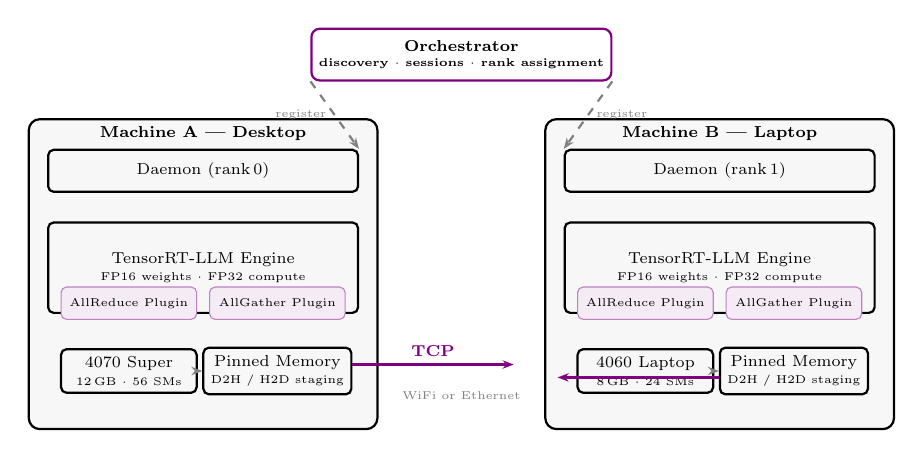
\begin{tikzpicture}[
    mach/.style={draw, rounded corners=4pt, minimum width=5.4cm,
                 minimum height=4.8cm, thick, fill=black!3},
    comp/.style={draw, rounded corners=2pt, minimum width=4.8cm,
                 minimum height=0.65cm, font=\scriptsize, align=center, thick},
    plug/.style={draw, rounded corners=2pt, minimum width=2.1cm,
                 minimum height=0.5cm, font=\tiny, align=center,
                 fill=violet!8, draw=violet!50},
    gpu/.style={draw, rounded corners=2pt, minimum width=2.1cm,
                minimum height=0.65cm, font=\scriptsize, align=center, thick},
    arr/.style={-{Stealth[length=4pt]}, thick},
    lbl/.style={font=\tiny, gray},
    scale=0.82, transform shape
  ]
  % Orchestrator
  \node[draw, rounded corners=3pt, minimum width=3.4cm, minimum height=0.8cm,
        font=\scriptsize\bfseries, align=center, draw=violet, thick]
    (orch) at (0,4.2) {Orchestrator\\[-1pt]{\tiny discovery $\cdot$ sessions $\cdot$ rank assignment}};

  % Machine A
  \node[mach] (ma) at (-4.0,0.8) {};
  \node[font=\scriptsize\bfseries, anchor=north] at (ma.north) {Machine A --- Desktop};
  \node[comp] (da) at (-4.0, 2.4) {Daemon (rank\,0)};
  \node[comp, minimum height=1.4cm] (ea) at (-4.0, 0.9) {TensorRT-LLM Engine\\{\tiny FP16 weights $\cdot$ FP32 compute}};
  \node[plug] (ar_a) at (-5.15, 0.35) {AllReduce Plugin};
  \node[plug] (ag_a) at (-2.85, 0.35) {AllGather Plugin};
  \node[gpu] (ga) at (-5.15, -0.7) {4070 Super\\{\tiny 12\,GB $\cdot$ 56 SMs}};
  \node[gpu] (pa) at (-2.85, -0.7) {Pinned Memory\\{\tiny D2H / H2D staging}};
  \draw[arr, gray] (ga.east) -- (pa.west);

  % Machine B
  \node[mach] (mb) at (4.0,0.8) {};
  \node[font=\scriptsize\bfseries, anchor=north] at (mb.north) {Machine B --- Laptop};
  \node[comp] (db) at (4.0, 2.4) {Daemon (rank\,1)};
  \node[comp, minimum height=1.4cm] (eb) at (4.0, 0.9) {TensorRT-LLM Engine\\{\tiny FP16 weights $\cdot$ FP32 compute}};
  \node[plug] (ar_b) at (2.85, 0.35) {AllReduce Plugin};
  \node[plug] (ag_b) at (5.15, 0.35) {AllGather Plugin};
  \node[gpu] (gb) at (2.85, -0.7) {4060 Laptop\\{\tiny 8\,GB $\cdot$ 24 SMs}};
  \node[gpu] (pb) at (5.15, -0.7) {Pinned Memory\\{\tiny D2H / H2D staging}};
  \draw[arr, gray] (gb.east) -- (pb.west);

  % Orchestrator arrows
  \draw[arr, gray, dashed] (orch.south west) -- node[left, lbl] {register} (da.north east);
  \draw[arr, gray, dashed] (orch.south east) -- node[right, lbl] {register} (db.north west);

  % TCP arrows
  \draw[arr, violet, thick] (pa.east) ++(0,0.1) -- node[above, font=\scriptsize\bfseries, violet] {TCP} ++(2.5,0) coordinate (tcpend);
  \draw[arr, violet, thick] ([yshift=-0.1cm]pb.west) -- ++(-2.5,0);
  \node[lbl, anchor=north] at (0,-0.9) {WiFi or Ethernet};
\end{tikzpicture}
\caption{System architecture.  The orchestrator manages topology; it does
not participate in data transfer.  Custom TensorRT plugins intercept
AllReduce/AllGather calls and route them through the TCP transport instead
of NCCL.  Pinned (page-locked) host memory enables DMA-speed GPU--host
transfers.}
\label{fig:architecture}
\end{figure*}

\paragraph{Orchestrator.}
A central orchestrator handles node registration, session matching, and
rank assignment.  Daemon nodes on each machine register with the
orchestrator, advertising their GPU capabilities (model, VRAM, SM count,
compute capability).  When compatible nodes come online, the orchestrator
creates a session and connects them.  The orchestrator does not participate
in data transfer---it only manages topology.

\paragraph{TCP transport and AllReduce.}
The custom transport replaces NCCL entirely.  Built on WinSock2 with a
POSIX socket fallback for Linux portability (untested).  Each rank
bootstraps by exchanging capability information, then establishing a
full-mesh of TCP connections.  Tensor data flows through a staged pipeline:
the GPU writes output to a pinned (page-locked) host buffer via
asynchronous D2H copy, the CPU sends that buffer over TCP to the peer, the
peer receives into its own pinned buffer, and a CUDA kernel reduces the
incoming tensor with the local partial result directly on GPU in FP32.
Each rank operates independently---no barrier, no assumption of symmetric
compute speed---which is what enables heterogeneous GPUs to participate in
the same AllReduce without protocol-level stalls.

\paragraph{Pinned memory architecture.}
The transport pre-allocates all host buffers at initialization using
\texttt{cudaHostAlloc} with \texttt{cudaHostAllocDefault}, page-locking
them in physical RAM\@.  Page-locked (pinned) memory bypasses the OS
virtual memory system, enabling DMA transfers between GPU and host at the
highest achievable PCIe bandwidth~\citep{nvidia2024cudaguide}---without
pinning, \texttt{cudaMemcpy} must first copy to an internal pinned staging
area, adding latency.  The transport maintains \textbf{four pinned
buffers} in a double-buffered configuration: two send/recv pairs that
alternate between consecutive AllReduce calls, preventing a situation where
the current call's recv overwrites the previous call's send data still in
flight.  A separate \textbf{GPU scratch buffer} handles the in-place
reduction case (where \texttt{send\_buf == recv\_buf}): peer data is
copied to scratch via H2D, local data remains in \texttt{recv\_buf}, and a
custom CUDA kernel sums them element-wise in FP32 precision.  No host-side
arithmetic ever touches the tensor data---all reduction is GPU-native.

\paragraph{Dual-socket connections.}
Each peer connection establishes two independent TCP sockets---one
dedicated for send, one for recv.  This enables truly simultaneous
bidirectional transfer: while rank~0 sends its tensor to rank~1, rank~1
simultaneously sends its tensor to rank~0, on separate sockets.  A single
TCP socket would serialize these operations (half-duplex at the application
layer even though TCP is full-duplex), doubling the exchange time.  With
dual sockets, the TCP exchange step completes in the time of one transfer,
not two.  Each socket is protected by its own mutex to prevent concurrent
access from the overlapped recv thread and the main send path.

% ---------- Figure 3: AllReduce Data Flow ----------
\begin{figure}[t]
\centering
\begin{tikzpicture}[
    step/.style={draw, rounded corners=2pt, minimum width=2.8cm,
                 minimum height=0.45cm, font=\tiny, align=center, thick},
    arr/.style={-{Stealth[length=3pt]}, thick, gray},
    lbl/.style={font=\tiny, gray},
    scale=0.85, transform shape
  ]
  % Rank 0
  \node[font=\tiny\bfseries] at (-1.8, 3.5) {Rank 0 (4070S)};
  \node[step] (gp0) at (-1.8, 3.0) {\ding{192} GPU partial};
  \node[step] (d2h0) at (-1.8, 2.2) {\ding{193} D2H $\to$ pinned (0.1\,ms)};
  \node[step, fill=violet!8, draw=violet!50] (red0) at (-1.8, 0.4)
    {\ding{196} GPU reduce (FP32)};

  % Rank 1
  \node[font=\tiny\bfseries] at (1.8, 3.5) {Rank 1 (4060L)};
  \node[step] (gp1) at (1.8, 3.0) {\ding{192} GPU partial};
  \node[step] (d2h1) at (1.8, 2.2) {\ding{193} D2H $\to$ pinned (0.1\,ms)};
  \node[step, fill=violet!8, draw=violet!50] (red1) at (1.8, 0.4)
    {\ding{196} GPU reduce (FP32)};

  % Arrows down
  \draw[arr] (gp0) -- (d2h0);
  \draw[arr] (gp1) -- (d2h1);
  \draw[arr] (d2h0) -- (red0);
  \draw[arr] (d2h1) -- (red1);

  % TCP arrows
  \draw[-{Stealth[length=3pt]}, violet, thick]
    ([yshift=2pt]d2h0.east) -- node[above, font=\tiny, violet]
    {\ding{194} TCP send} ([yshift=2pt]d2h1.west);
  \draw[-{Stealth[length=3pt]}, violet, thick]
    ([yshift=-2pt]d2h1.west) -- node[below, font=\tiny, violet]
    {\ding{195} TCP recv} ([yshift=-2pt]d2h0.east);

  \node[lbl, align=center] at (0, -0.2) {No barrier---slower rank sets the pace.\\Both ranks execute simultaneously.};
\end{tikzpicture}
\caption{AllReduce data flow for TP=2 direct exchange.  Both ranks
simultaneously send/recv on dual TCP sockets, then reduce on GPU in FP32.
For $N>2$, the exchange becomes a ring
AllReduce~\citep{gibiansky2017hpc,patarasuk2009bandwidth}.}
\label{fig:allreduce-flow}
\end{figure}

For \textbf{TP=2} (the common case), AllReduce is optimized as a direct
exchange: both ranks simultaneously send their full tensor over dual TCP
sockets, receive the peer's tensor into a pinned recv buffer, and sum on
GPU via the custom FP32 kernel.  No ring topology---just one round trip.
For \textbf{larger topologies} ($N>2$ GPUs), the system implements a ring
AllReduce~\citep{gibiansky2017hpc} in two phases: reduce-scatter followed
by all-gather.  Total data transferred scales optimally at
$2(N\!-\!1)/N \times \text{tensor\_size}$~\citep{patarasuk2009bandwidth}.
Send and receive are overlapped to pipeline TCP I/O with GPU computation.
The ring path is implemented but untested beyond TP=2; all benchmarks in
this paper use the direct exchange.

\paragraph{TensorRT plugin integration.}
TensorRT-LLM's multi-GPU support is hardcoded to NCCL---every AllReduce,
AllGather, and ReduceScatter operation in the engine graph calls into
NCCL's collective communication library.  There is no plugin interface or
abstraction layer for swapping the communication backend.  To replace NCCL
with our TCP transport, we implemented custom TensorRT
\texttt{IPluginV2DynamicExt} plugins from scratch in C++---one for each
collective operation.  These plugins register under the same operation
names that TRT-LLM emits during engine compilation, so they intercept
every collective call at execution time without modifying TRT-LLM's model
definitions, graph construction, or weight loading.  The engine graph is
unchanged; only the communication backend is swapped.

This required solving several integration challenges.  TensorRT's plugin
initialization order does not guarantee that the TCP transport is connected
when the engine loads---the plugins use lazy initialization, acquiring the
transport singleton on first \texttt{enqueue()} rather than at
\texttt{initialize()} time.  During engine compilation, TensorRT profiles
each plugin with test data to select optimal execution tactics---a
no-transport fallback (shifted-add) prevents TRT from
dead-code-eliminating the AllReduce operations, which would silently strip
them from the execution graph.  The plugins handle FP16, FP32, BF16, INT8,
INT32, INT64, and FP8 data types, matching TRT-LLM's full dtype coverage
for collective operations.

% ============================================================
\section{TensorRT-LLM on Windows}\label{sec:windows}

NVIDIA discontinued Windows support for TensorRT-LLM\@.  We restored it on
v0.12.0, the last release with partial Windows compatibility, and the
latest at time of development.  This is a prerequisite for consumer
deployment: the vast majority of the 100M+ RTX GPUs cited in
\S\ref{sec:intro} run Windows, and requiring Linux would exclude most of
the target hardware.

The port required patches at four layers of the build system:
\textbf{Package management}---Conan dependency profiles assumed Linux
toolchains; we wrote Windows-native profiles for all C++ dependencies.
\textbf{FMHA kernel compilation}---fused multi-head attention kernels used
GCC-specific intrinsics and POSIX paths; we ported these to MSVC with
equivalent CUDA intrinsics.
\textbf{Python bindings}---nanobind's build configuration assumed Unix
shared library conventions; we patched the CMake targets for Windows DLL
generation.
\textbf{MSVC/CUDA interop}---the CUDA toolkit and MSVC have different C++
ABI expectations for exception handling and name mangling; we resolved
linking failures across the toolchain boundary.

The result is a native Windows build that compiles and executes
TensorRT-LLM inference engines---the full set of NVIDIA's 1,500+
hand-tuned CUDA kernels for attention, GEMM, and quantization---without
WSL, Docker, or any Linux compatibility layer.

% ============================================================
\section{Experimental Evaluation}\label{sec:eval}

We demonstrated tensor parallelism across two heterogeneous GPUs on
separate machines:

\begin{itemize}[nosep,leftmargin=*]
  \item \textbf{Rank 0:} NVIDIA RTX 4070 Super---12\,GB VRAM, 56 SMs
  \item \textbf{Rank 1:} NVIDIA RTX 4060 Laptop---8\,GB VRAM, 24 SMs
\end{itemize}

These GPUs differ in VRAM, SM count, and clock speed---a configuration
NCCL cannot support.  Both GPUs share the same SM architecture (Ada
Lovelace, sm\_89)---heterogeneous TP has only been confirmed across GPUs
with identical SM architectures.  Cross-architecture TP (\eg, Ampere +
Ada) within the same TP group remains untested and may introduce divergence
from differing instruction-level behavior.  In MoE configurations,
different experts can run on different architectures freely since experts
never AllReduce with each other---the constraint applies only within each
expert's TP group.

\paragraph{Experimental setup.}
\textbf{Software:} NVIDIA TensorRT-LLM v0.12.0 (custom Windows build),
CUDA Toolkit 12.6, cuDNN 9.3, TensorRT 10.4, Python~3.12, Windows~11 Pro
on both machines.  Engines built with \texttt{trtllm-build} using TP=2,
FP16 weights with FP32 AllReduce accumulation.
\textbf{Network:} WiFi tests used 802.11ac (5\,GHz), measured ping
316\,ms round-trip under load.  Ethernet tests used gigabit (1000BASE-T)
via consumer router, measured ping 0.5--1\,ms.
\textbf{Methodology:} All latency measurements are per-token generation
time during autoregressive decoding, measured after a 5-token warm-up
period to ensure CUDA kernels are JIT-compiled and GPU clocks are boosted.
Each reported number is the median of 20 consecutive tokens.  Throughput is
computed as $1/\text{latency}$.  AllReduce timing breakdowns use CUDA
event-based instrumentation inserted at each stage of the D2H $\to$ TCP
$\to$ H2D $\to$ reduce pipeline.

\subsection{Correctness---TinyLlama 1.1B}

TinyLlama 1.1B (22 layers, FP32) was split horizontally, with each rank
holding half the weights.  Every transformer layer synchronizes via our
custom TCP AllReduce with FP32 accumulation.  Verified outputs across both
ranks:

\begin{itemize}[nosep,leftmargin=*]
  \item \textbf{``1+1=''} $\rightarrow$ ``2'' --- both ranks agree \checkmark
  \item \textbf{``The capital of France is''} $\rightarrow$ ``Paris'' --- both ranks agree \checkmark
  \item \textbf{``A cat is a''} $\rightarrow$ ``domestic'' --- both ranks agree \checkmark
\end{itemize}

Identical outputs from two different GPUs, on two different machines.
FP32 GPU-native reduction is what makes this possible---without it,
accumulated precision loss corrupts the output by layer~15.

\subsection{Scale---Mistral 7B}

To prove the architecture scales beyond toy models, we built and deployed
\textbf{Mistral 7B Instruct}---a 7 billion parameter model with 32
transformer layers, grouped-query attention (8 KV heads), and 14\,GB of
FP16 weights.  This model \textbf{cannot fit on either GPU alone}: the
4070~Super has 12\,GB, the 4060~Laptop has 8\,GB.  Without tensor
parallelism, this model simply doesn't run on consumer hardware with less
than 16\,GB VRAM\@.

With TP=2 across both machines, Mistral 7B produces coherent output:

\begin{quote}
\textbf{``What is the capital of France?''} $\rightarrow$ ``The capital of
France is Paris.''\\
Generation latency: \textbf{80\,ms/token (12.5\,tok/s)} over gigabit
ethernet with KV cache + overlapped AllReduce.
\end{quote}

\subsection{Benchmark Data}

% ---------- Table 3: Performance ----------
\begin{table}[t]
\centering
\caption{Performance comparison across configurations.}
\label{tab:benchmarks}
\smallskip
\resizebox{\columnwidth}{!}{%
\begin{tabular}{@{}lrrl@{}}
\toprule
Configuration & Latency & Tput & Notes \\
\midrule
llama.cpp --- 4070S single & 3.4\,ms & 295\,t/s & Q8, single GPU baseline \\
BMRT TP=2 --- localhost & 8.1\,ms & 123\,t/s & TinyLlama, no network \\
BMRT TP=2 --- WiFi & 277\,ms & 3.6\,t/s & TinyLlama, 316\,ms ping \\
BMRT TP=2 --- Ethernet & 276\,ms & 3.6\,t/s & TinyLlama, 1\,ms ping \\
BMRT TP=2 --- Mistral (early) & 185\,ms & 5.4\,t/s & Overlap, 49\,KB payload \\
\textbf{BMRT TP=2 --- Mistral} & \textbf{80\,ms} & \textbf{12.5\,t/s}
  & \textbf{KV cache, 8\,KB payload} \\
\bottomrule
\end{tabular}}
\end{table}

\subsection{Analysis: Network Latency vs.\ Synchronization Overhead}\label{sec:eval-analysis}

\textbf{Before overlap optimization:} gigabit ethernet (1\,ms ping) and
WiFi (316\,ms ping) produced identical throughput---276\,ms vs.\ 277\,ms
per token.  A $300\times$ improvement in raw network latency yielded zero
improvement in token generation speed.  This initially appeared to
contradict the assumption that network latency makes per-layer
synchronization infeasible.

Instrumentation revealed why.  In the synchronous (pre-overlap)
implementation, each AllReduce call spent 1.5--5\,ms waiting for GPU
compute to finish before any network transfer began.  This synchronization
wait dominated the per-call cost, masking the actual network transfer time.
WiFi and ethernet produced identical results because neither was the
bottleneck---the GPU sync wait was.

\textbf{After overlap optimization:} we start the TCP recv in a background
thread \emph{before} waiting for GPU compute, so recv runs in parallel
with the sync wait.  With double-buffered pinned memory to prevent
send/recv conflicts, the overlapped AllReduce hides recv time behind the
sync wait on the critical path.

% ---------- Figure 4: Timeline ----------
\begin{figure}[t]
\centering
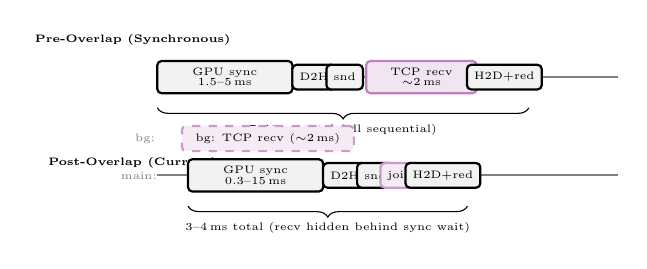
\begin{tikzpicture}[
    blk/.style={draw, rounded corners=1.5pt, minimum height=0.4cm,
                font=\tiny, align=center, thick},
    lbl/.style={font=\tiny, gray},
    scale=0.78, transform shape
  ]
  % --- Pre-overlap ---
  \node[font=\tiny\bfseries] at (-0.4, 2.2) {Pre-Overlap (Synchronous)};
  \draw[gray, thick] (0,1.6) -- (7.5,1.6);
  \node[blk, minimum width=2.2cm, fill=black!5] (sync1) at (1.1,1.6)
    {GPU sync\\[-1pt]1.5--5\,ms};
  \node[blk, minimum width=0.5cm, fill=black!5] (d2h1) at (2.55,1.6) {D2H};
  \node[blk, minimum width=0.5cm, fill=black!5] (snd1) at (3.05,1.6) {snd};
  \node[blk, minimum width=1.8cm, fill=violet!10, draw=violet!50] (rcv1) at (4.3,1.6)
    {TCP recv\\[-1pt]$\sim$2\,ms};
  \node[blk, minimum width=0.8cm, fill=black!5] (red1) at (5.65,1.6) {H2D+red};
  % Brace
  \draw[decorate, decoration={brace, amplitude=4pt, mirror}]
    (0,1.1) -- (6.05,1.1) node[midway, below=4pt, font=\tiny] {7--10\,ms total (all sequential)};

  % --- Post-overlap ---
  \node[font=\tiny\bfseries] at (-0.4, 0.2) {Post-Overlap (Current)};
  % bg thread
  \node[blk, minimum width=2.8cm, fill=violet!8, draw=violet!40, dashed]
    (bgrcv) at (1.8,0.6) {bg: TCP recv ($\sim$2\,ms)};
  \node[lbl] at (-0.2,0.6) {bg:};
  % main thread
  \draw[gray, thick] (0,0) -- (7.5,0);
  \node[lbl] at (-0.3,0) {main:};
  \node[blk, minimum width=2.2cm, fill=black!5] (sync2) at (1.6,0)
    {GPU sync\\[-1pt]0.3--15\,ms};
  \node[blk, minimum width=0.5cm, fill=black!5] (d2h2) at (3.05,0) {D2H};
  \node[blk, minimum width=0.5cm, fill=black!5] (snd2) at (3.55,0) {snd};
  \node[blk, minimum width=0.4cm, fill=violet!8, draw=violet!40] (join) at (3.95,0) {join};
  \node[blk, minimum width=0.8cm, fill=black!5] (red2) at (4.65,0) {H2D+red};
  % Brace
  \draw[decorate, decoration={brace, amplitude=4pt, mirror}]
    (0.5,-0.5) -- (5.05,-0.5) node[midway, below=4pt, font=\tiny]
    {3--4\,ms total (recv hidden behind sync wait)};
\end{tikzpicture}
\caption{AllReduce timeline before and after overlap optimization.
Pre-overlap: all stages sequential (7--10\,ms).  Post-overlap: TCP recv
runs on a background thread during GPU sync wait; when sync\_wait $>$
recv\_time, the recv adds zero time to the critical path.}
\label{fig:timeline}
\end{figure}

When the GPU sync wait (0.3--15\,ms) exceeds the recv time ($\sim$2\,ms),
the recv completes before the main thread needs it---the join is instant
and recv adds zero time to the critical path.  The effective per-call cost
becomes: $\text{sync\_wait} + \text{D2H}~(0.1\,\text{ms}) +
\text{send}~(0.1\,\text{ms}) + \text{join}~(0\,\text{ms}) +
\text{H2D+reduce}~(0.3\,\text{ms}) \approx \text{sync\_wait} +
0.5\,\text{ms}$.  At 3--4\,ms per call $\times$ 64 calls per token
(Mistral 7B, 32 layers with AllReduce + AllGather), this yields
$\sim$185\,ms/tok.

This reduced per-call AllReduce from 7--10\,ms to 3--4\,ms and improved
Mistral 7B generation from 293\,ms to \textbf{185\,ms/tok (5.4\,tok/s)}---a
37\% latency reduction.  Full layer-level pipelining (deferring
recv+reduce to the next AllReduce call) was attempted but breaks TRT-LLM's
buffer contract---the engine expects the reduced result in
\texttt{recv\_buf} before \texttt{allReduce()} returns.

\paragraph{KV cache effect on AllReduce payload.}
With correct KV caching, the generation phase processes a single token per
step instead of re-computing the full context.  This shrinks the AllReduce
payload from $\sim$49\,KB (full activation tensor) to \textbf{8\,KB}
(single-token hidden state).  At 8\,KB, each AllReduce call completes in
$\sim$1.2\,ms---down from 3--4\,ms at 49\,KB\@.  Over 64 calls per token,
this reduces AllReduce overhead from $\sim$224\,ms to $\sim$77\,ms.
Combined with faster single-token GPU compute, generation latency drops to
\textbf{80\,ms/tok (12.5\,tok/s)}---a $2.3\times$ improvement over the
pre-KV-cache measurement.

\paragraph{Optimization trajectory.}
The three benchmark stages tell a story about where the remaining headroom
lies:

\begin{enumerate}[nosep,leftmargin=*]
  \item \textbf{293\,ms/tok} --- Synchronous AllReduce.  Recv blocks the
    critical path.  GPU sync wait (1.5--5\,ms) + network transfer
    ($\sim$2\,ms) = 7--10\,ms per call $\times$ 64 calls.
  \item \textbf{185\,ms/tok} --- Overlapped AllReduce.  Recv runs during
    GPU sync wait.  Per-call cost drops to 3--4\,ms.  A 37\% latency
    reduction from hiding I/O behind compute.
  \item \textbf{80\,ms/tok} --- KV cache fix.  Generation-phase payload
    shrinks from 49\,KB to 8\,KB\@.  Per-call cost drops to $\sim$1.2\,ms.
    A further 57\% reduction from sending less data.
\end{enumerate}

Each stage removed a different bottleneck: first the blocking recv, then
the payload size.  The remaining bottleneck is the GPU sync wait itself
($\sim$0.7\,ms per call), which is the time for each layer's TensorRT
compute to finish---the irreducible cost of the model's arithmetic.
Further gains require either reducing per-layer compute (quantization,
pruning) or overlapping the next layer's compute with the current layer's
reduction (layer-level pipelining, which we attempted but is blocked by
TRT-LLM's buffer contract).  Larger models improve the ratio further: more
compute per layer means more sync wait to hide communication behind,
making AllReduce overhead a smaller fraction of per-token cost.

To contextualize: 12.5\,tokens/second is not competitive with single-GPU
inference on a model that fits in VRAM---\texttt{llama.cpp} on one
4070~Super runs a quantized model at 295\,tok/s.  But TP and single-GPU
address fundamentally different constraints.  Single-GPU runs models that
fit on one card.  TP splits a model that \textbf{cannot fit on any single
GPU} across several for capability---and at 12.5\,tok/s, the output
streams faster than a human reads.  The throughput is practical for
interactive use, and the correctness result---identical output from
mismatched GPUs over a commodity network---is the primary contribution.

% ============================================================
\section{Limitations}\label{sec:limitations}

Correctness is proven across two model scales.  Overlapped AllReduce
(\S\ref{sec:eval-analysis}) improved Mistral 7B latency from 293\,ms to
80\,ms/tok.  The remaining optimizations:

\textbf{Further computation-communication overlap} --- the current
implementation overlaps TCP recv with GPU sync wait by starting recv in a
background thread.  Full layer-level pipelining---deferring the previous
layer's recv+reduce while the next layer's compute begins---was attempted
but breaks TRT-LLM's buffer contract.  Achieving this would require
modifying TensorRT's execution model or introducing a shadow buffer scheme.

\textbf{Larger models improve the ratio} --- Mistral 7B (32 layers,
14\,GB) achieves nearly the same per-token latency as TinyLlama (22
layers, 2\,GB) despite $10\times$ more parameters.  Each layer has more
compute relative to the fixed AllReduce overhead.  At 70B+ parameters, the
AllReduce cost becomes a rounding error---exactly where TP shines.

\textbf{Same SM architecture required within a TP group} ---
heterogeneous TP has been confirmed only across GPUs sharing the same SM
architecture (Ada Lovelace, sm\_89).  Cross-architecture pairs (\eg,
Ampere sm\_86 + Ada sm\_89) within the same TP group remain untested.
In MoE configurations, this constraint applies only within each expert's
TP group---different experts can run on different architectures since they
never AllReduce with each other.

\textbf{Asymmetric weight splitting} --- currently, TP splits weight
matrices evenly.  With heterogeneous GPUs, proportional splitting (more
columns to the GPU with more VRAM) would allow larger models to fit across
mismatched hardware.  The transport and reduction layers are already
agnostic to split ratios.

\textbf{Concurrent serving} --- dense TP locks all ranks for every token.
The current system serves one user at a time.  Continuous
batching---processing multiple users' tokens in the same forward
pass---would amortize AllReduce overhead across $N$ users while growing
the payload only linearly ($8\,\text{KB} \times N$).  TRT-LLM supports
this on Linux via its C++ executor; enabling it over our TCP transport
requires adapting the scheduling logic.  MoE architectures
(\S\ref{sec:future}) solve this structurally: only 2 of 8 experts activate
per token, so 75\% of the mesh can serve other users concurrently without
batching.

We prioritized proving correctness over the most challenging
transport---WiFi between consumer laptops.  The benchmarks demonstrate
that the transport is already saturated: faster networks yield no
throughput improvement because the network is not the bottleneck.
\textbf{The remaining gains lie in overlapping compute with communication
and in model architectures that reduce synchronization points---both
engineering optimizations rather than open research problems.}

% ============================================================
\section{Future Work}\label{sec:future}

\subsection{Mixture-of-Experts and Edge Compute}

Dense transformer models are the worst case for edge tensor
parallelism---every layer requires AllReduce across all ranks, every
token.  But the industry is moving to \textbf{Mixture-of-Experts (MoE)}
architectures, and this changes the math entirely.

In a MoE model like Mixtral~\citep{jiang2024mixtral}, each transformer
layer contains multiple expert sub-networks, but only 2 of 8 experts
activate per token.  A gating network routes each token to its
best-matching experts.  The rest stay idle.  This means most of the
model's parameters exist but don't participate in any given forward
pass---a property that is inefficient in a data center but
\textbf{advantageous for a distributed compute mesh}.

Instead of splitting one dense model across GPUs that must synchronize
every layer, each expert lives on a different node.  A token arrives, the
gate selects two experts, and only those two nodes compute.  No AllReduce
across all ranks---just point-to-point communication between the gate and
the selected experts.  The per-layer synchronization bottleneck that makes
dense TP painful over WiFi largely disappears.

The compute mesh topology becomes an advantage, not a liability.  Experts
can be placed geographically---routed to the nearest available GPU with
that expert hot in VRAM, like a CDN for inference.  A gamer in Jakarta
holds Expert~3, a researcher in Nairobi holds Expert~7.  A token that
needs both pays two point-to-point hops, not a global AllReduce.

The two parallelism strategies also compose.  If a single expert is too
large for one GPU, it can be tensor-parallelized across nearby GPUs---TP
within the expert, expert parallelism across the mesh.  This creates two
tiers of communication: \textbf{EP across the internet} for routing tokens
to the right expert (point-to-point, latency-tolerant, one hop), and
\textbf{TP across local GPUs} for computing within the expert (AllReduce
over ethernet at 0.1\,ms, not WiFi at 5\,ms).  Since only 2 of 8 experts
activate per token, 75\% of the mesh is idle for any given
request---available to serve other tokens concurrently.

% ---------- Figure 5: MoE diagram ----------
\begin{figure}[t]
\centering
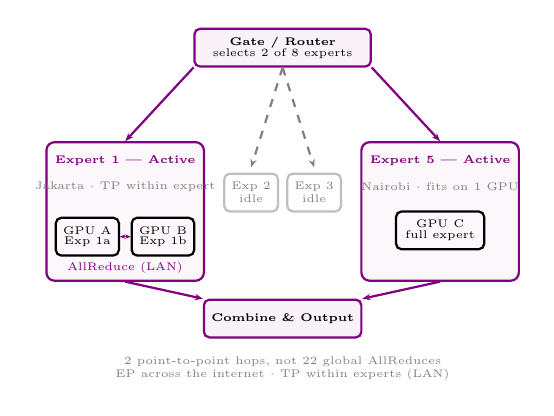
\begin{tikzpicture}[
    box/.style={draw, rounded corners=2pt, minimum height=0.6cm,
                font=\tiny, align=center, thick},
    exp/.style={draw, rounded corners=3pt, minimum width=2.5cm,
                minimum height=2.2cm, thick},
    arr/.style={-{Stealth[length=3pt]}, thick},
    lbl/.style={font=\tiny, gray},
    scale=0.8, transform shape
  ]
  % Gate
  \node[box, minimum width=2.8cm, draw=violet, fill=violet!5]
    (gate) at (0,3.8) {\textbf{Gate / Router}\\[-1pt]selects 2 of 8 experts};

  % Expert 1 (active)
  \node[exp, draw=violet, fill=violet!3] (e1) at (-2.5,1.2) {};
  \node[font=\tiny\bfseries, violet] at (-2.5,2.0) {Expert 1 --- Active};
  \node[lbl] at (-2.5,1.6) {Jakarta $\cdot$ TP within expert};
  \node[box, minimum width=0.9cm] (g1a) at (-3.1,0.8) {GPU A\\[-1pt]{\tiny Exp 1a}};
  \node[box, minimum width=0.9cm] (g1b) at (-1.9,0.8) {GPU B\\[-1pt]{\tiny Exp 1b}};
  \draw[{Stealth[length=2pt]}-{Stealth[length=2pt]}, violet, dashed]
    (g1a.east) -- (g1b.west);
  \node[lbl, violet] at (-2.5,0.3) {AllReduce (LAN)};

  % Expert 5 (active)
  \node[exp, draw=violet, fill=violet!3] (e5) at (2.5,1.2) {};
  \node[font=\tiny\bfseries, violet] at (2.5,2.0) {Expert 5 --- Active};
  \node[lbl] at (2.5,1.6) {Nairobi $\cdot$ fits on 1 GPU};
  \node[box, minimum width=1.4cm] (g5) at (2.5,0.9) {GPU C\\[-1pt]{\tiny full expert}};

  % Idle experts
  \node[box, draw=gray!50, text=gray, minimum width=0.7cm] at (-0.5,1.5) {Exp 2\\idle};
  \node[box, draw=gray!50, text=gray, minimum width=0.7cm] at (0.5,1.5) {Exp 3\\idle};

  % Gate arrows
  \draw[arr, violet] (gate.south west) -- (e1.north);
  \draw[arr, violet] (gate.south east) -- (e5.north);
  \draw[arr, gray, dashed] (gate.south) -- (-0.5,1.9);
  \draw[arr, gray, dashed] (gate.south) -- (0.5,1.9);

  % Combine
  \node[box, minimum width=2.5cm, draw=violet, fill=violet!5]
    (comb) at (0,-0.5) {\textbf{Combine \& Output}};
  \draw[arr, violet] (e1.south) -- (comb.north west);
  \draw[arr, violet] (e5.south) -- (comb.north east);

  \node[lbl, align=center] at (0,-1.3) {2 point-to-point hops, not 22 global AllReduces\\
    EP across the internet $\cdot$ TP within experts (LAN)};
\end{tikzpicture}
\caption{MoE hybrid parallelism.  The gate routes each token to 2 of 8
experts.  Expert parallelism (EP) uses point-to-point TCP across the
internet; tensor parallelism (TP) uses AllReduce within local GPU clusters.
75\% of experts are idle per token---available for concurrent serving.}
\label{fig:moe}
\end{figure}

\textbf{Data center architecture is overprovisioned for MoE.} Dense
transformers activate every parameter on every token---they fully utilize
NVLink's 900\,GB/s bandwidth and justify the cost of keeping every GPU in
a DGX node busy.  MoE inverts this: 75\% of parameters are idle per token,
and the communication pattern is sparse point-to-point, not dense
AllReduce.  Data centers compensate by batching aggressively, but this
requires sustained high request volume.  A \$3M GB200 NVL72 rack has 75\%
of its 13.8\,TB VRAM idle per token.  A mesh inverts the cost structure:
idle VRAM costs nearly nothing because it sits in consumer hardware that
would otherwise be sleeping, and expert routing needs only commodity TCP\@.
Moreover, data centers scale beyond NVLink via pipeline
parallelism---a degraded mechanism that increases sequential depth and
introduces bubbles.  MoE on a mesh scales via expert parallelism: each
expert occupies its own node(s), aggregate VRAM grows linearly with mesh
size ($100~\text{nodes} \times 12\,\text{GB} = 1.2\,\text{TB}$), and
per-token communication cost does not increase.  \textbf{Data centers
scale capacity by adding pipeline stages.  The mesh scales capacity by
adding participants.  One degrades utilization; the other does not.}

\paragraph{Mesh formation.}
The orchestrator already solves the assignment problem for dense TP: nodes
register, advertise GPU capabilities, and receive rank assignments.  MoE
extends this with expert placement.  When a node joins the mesh, the
orchestrator evaluates its VRAM capacity, network latency to existing
nodes, and which experts are underserved---then assigns one or more experts
and pushes the corresponding weight shards.  If an expert is too large for
a single GPU, the orchestrator groups nearby low-latency nodes into a TP
group for that expert, exactly as it does today for dense models.

\paragraph{Redundancy and fault tolerance.}
Dense TP has no tolerance for node failure---if any rank drops, the entire
inference pass is invalid.  MoE on a mesh offers a structural alternative.
Since only 2 of 8 experts activate per token and 75\% of nodes are idle at
any moment, the orchestrator can maintain \textbf{replicated
experts}---the same expert weights loaded on multiple nodes in different
locations.  When the orchestrator's heartbeat detects a node failure, it
re-routes subsequent tokens to a surviving replica.  No checkpoint, no
restart, no lost inference state---the next token simply goes elsewhere.

\paragraph{Concurrent serving.}
Dense TP locks every GPU into a single inference pass.  MoE on a mesh does
not: since only 2 of 8 experts activate per token, 75\% of nodes can
simultaneously serve other users' tokens.  Multiple inference requests flow
through the mesh concurrently without explicit batching or model
replication---the sparsity that makes MoE parameter-efficient also makes
it serving-efficient.

Our transport layer already supports arbitrary world sizes and
rank-to-rank communication.  The infrastructure for MoE routing is the
same TCP mesh we built for tensor parallelism---the difference is traffic
pattern, not protocol.  \textbf{Dense TP validates the transport layer;
MoE architectures are where it achieves practical scalability.}

\subsection{Distributed KV Cache}

Foundation models increasingly support context windows of 128K--1M+
tokens.  The KV cache required to serve these contexts grows linearly with
sequence length---at 128K tokens, Mistral 7B's KV cache alone consumes
4--8\,GB per GPU, approaching or exceeding the total VRAM of consumer
hardware.  This is the next wall after model size: even when tensor
parallelism enables a model's weights to fit across multiple GPUs, a long
context window can exhaust the remaining VRAM on the smallest device.

Existing solutions trade latency for capacity.
FlexGen~\citep{sheng2023flexgen} offloads KV cache to CPU RAM and disk,
solving the memory problem but adding 10--50\,ms per page fault.  Ring
Attention~\citep{liu2023ring} distributes the sequence across devices,
requiring all devices to participate in every attention computation---a
global synchronization cost that scales with world size.  PagedAttention
(vLLM) manages KV cache as virtual memory pages on a single GPU but cannot
help when that GPU is full.

Our mesh architecture enables a different approach: \textbf{distributed KV
cache across idle nodes}.  The orchestrator already tracks every node's GPU
model, VRAM capacity, and current utilization.  The TCP transport already
moves tensors between GPUs with pinned-memory staging.  In an MoE
configuration, 75\% of expert nodes are idle for any given token---their
VRAM is empty and available.  Instead of evicting old KV entries to CPU or
dropping context, we propose paging them to peer GPUs in the mesh that
have free VRAM\@.

This creates a three-tier memory hierarchy for KV cache:

\begin{itemize}[nosep,leftmargin=*]
  \item \textbf{Tier 1---Local GPU VRAM} (hot): Recent tokens, zero
    additional latency.
  \item \textbf{Tier 2---Peer GPU VRAM} (warm): Older tokens paged to
    idle nodes.  Retrieval cost is one TCP round trip (1--5\,ms over
    ethernet)---slower than local VRAM but faster than disk I/O
    (10--50\,ms).
  \item \textbf{Tier 3---CPU RAM / disk} (cold): Oldest tokens, last
    resort.
\end{itemize}

The critical difference from existing offloading schemes is that Tier~2
uses \textbf{GPU VRAM on peer nodes}, not local CPU RAM\@.  A fetch from
peer GPU VRAM over ethernet is a DMA-speed copy on both ends with a
network hop in between---the same staged pipeline (GPU $\to$ pinned host
$\to$ TCP $\to$ pinned host $\to$ GPU) already proven in our AllReduce
implementation.  Unlike Ring Attention, only the node that needs a specific
KV block fetches it---no global synchronization, just point-to-point
retrieval.

In MoE configurations, this composes naturally with expert routing.  The
gate routes a token to two active experts; the remaining six expert nodes
are idle, their combined VRAM forming a distributed memory pool.  The same
orchestrator that routes computation can route KV cache
placement---assigning pages to the nearest node with free VRAM, like a CDN
for memory.

Three prerequisites make this approach viable: (1)~an orchestrator with
real-time visibility into per-node VRAM utilization, (2)~a transport layer
capable of GPU-to-GPU tensor transfer across the network, and (3)~idle
nodes with empty VRAM available as storage.  Our system already satisfies
all three.  The remaining work is a cache eviction policy (LRU with
locality-aware placement) and integration with TensorRT-LLM's attention
kernels to support non-contiguous KV cache reads.  \textbf{The same mesh
that routes computation can also route memory, reducing dependence on
centralized cloud infrastructure.}

% ============================================================
\section{Conclusion}\label{sec:conclusion}

We presented the first implementation of heterogeneous tensor parallelism
across consumer GPUs on separate machines over commodity TCP networks.  By
solving two problems that blocked prior attempts---precision loss during
networked AllReduce and synchronization failure across mismatched
GPUs---we demonstrated that tensor parallelism is feasible outside of
homogeneous data center hardware.  Our benchmarks revealed that in
synchronous tensor parallelism, GPU synchronization overhead---not network
latency---is the dominant bottleneck: a $300\times$ improvement in network
latency yielded zero improvement in throughput.  Overlapping TCP recv with
GPU synchronization reduced per-call AllReduce cost by 50--60\%.  Combined
with correct KV caching---which shrinks the generation-phase AllReduce
payload from 49\,KB to 8\,KB---Mistral 7B generation improved from
293\,ms to \textbf{80\,ms/tok (12.5\,tok/s)}.

The system produces identical output from two different GPUs (RTX~4070
Super and RTX~4060 Laptop) running Mistral 7B---a 14\,GB model too large
for either GPU alone---over gigabit ethernet.  The industry's shift toward
Mixture-of-Experts architectures, where only a fraction of parameters
activate per token, structurally favors distributed meshes over centralized
data centers: expert routing requires only point-to-point communication
over commodity networks, not AllReduce over NVLink, and data centers scale
past their NVLink domains via pipeline parallelism---a degraded mechanism
that reintroduces the bubbles and idle GPUs that tensor parallelism was
designed to eliminate.  A mesh scales via expert parallelism, which does
not degrade.  Dense tensor parallelism proved the transport works.
Mixture-of-Experts is where it becomes practical.

% ============================================================
\bibliography{references}

\end{document}
